
\section*{Problem  Set 3}


\begin{mdframed}

\includegraphics[width=400pt]{img/algebra--nf--2-179c.png}
\end{mdframed}

[I'll let you know when I've updated this document with this answer.]

~\\~\\
{\bf Section 1.6}\\

\begin{mdframed}
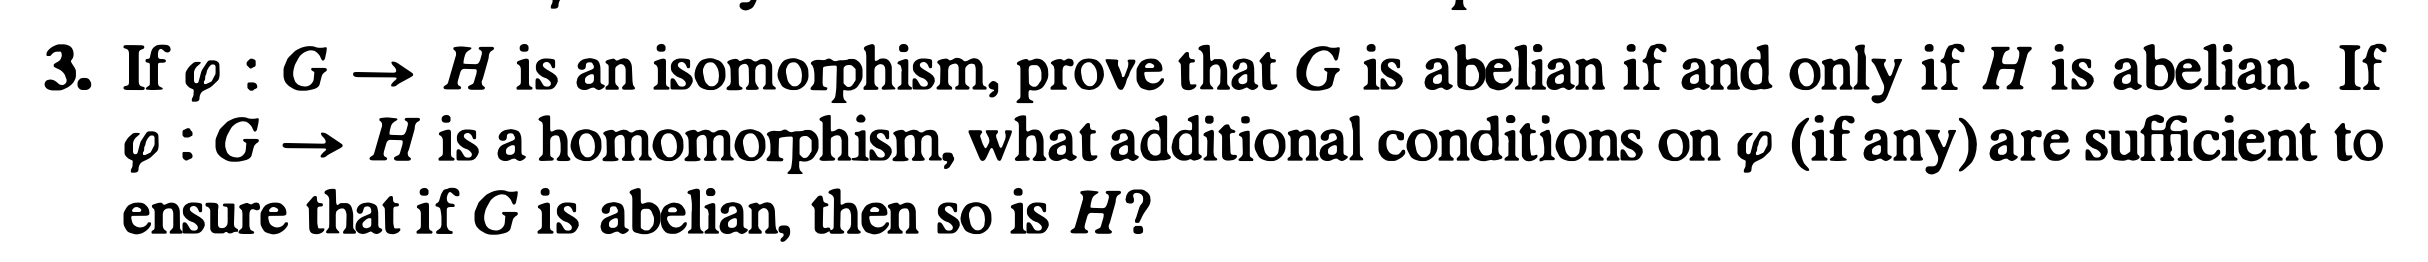
\includegraphics[width=400pt]{img/abstract-algebra--nf--3-4cd9.png}
\end{mdframed}

\begin{proof}
  Let $G$ be abelian and let $h_1, h_2 \in H$. Since $\varphi$ is an isomorphism it is surjective, hence
  there exists $g_1, g_2 \in G$ such that $h_1 = \varphi(g_1)$ and $h_2 = \varphi(g_2)$. Therefore
  \begin{align*}
    h_1h_2 &= \varphi(g_1)\varphi(g_2)\\
           &= \varphi(g_1g_2)       &&\text{$\phi$ is a homomorphism}\\
           &= \varphi(g_2g_1)       &&\text{$G$ is abelian }\\
           &= \varphi(g_2)\varphi(g_1)    &&\text{$\phi$ is a homomorphism}\\
           &= h_2h_1.
  \end{align*}

  Conversely, let $H$ be abelian and let $g_1, g_2 \in G$. Since $\varphi$ is an isomorphism,
  $\varphi^{-1}$ exists and is an isomorphism. It follows that $g_1g_2 = g_2g_1$ by the same argument as
  above, with the following formal substitutions:
  \begin{align*}
    G &\longleftrightarrow H \\
    g_1, g_2 &\longleftrightarrow h_1, h_2 \\
    \varphi &\longrightarrow \varphi^\1.
  \end{align*}
\end{proof}

{\bf Sufficient conditions on $\varphi$ to ensure that ($G$ abelian $\implies H$ abelian)\\}\\
In the forwards direction it was sufficient for $\varphi$ to be a surjective homomorphism; we didn't
require it to be an isomorphism (injective).

~\\~\\
\begin{mdframed}

\includegraphics[width=400pt]{img/abstract-algebra--nf--3-89f3.png}
\end{mdframed}

[I'll let you know when I've updated this document with this answer.]

\begin{mdframed}
\newpage
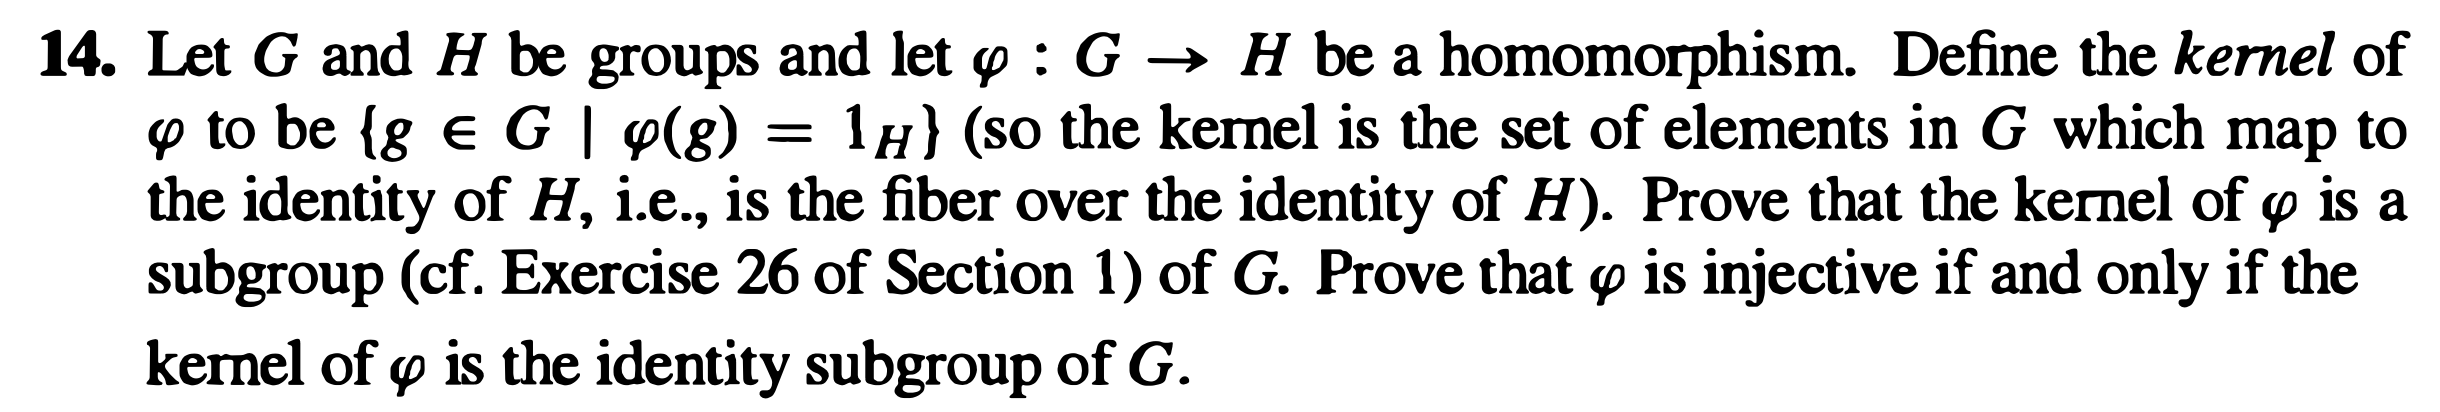
\includegraphics[width=400pt]{img/abstract-algebra--nf--3-b601.png}
\end{mdframed}


\begin{proof}~\\
  {\bf Contains identity:}\\
  Let $g \in G$. Since $\varphi$ is a homomorphism we have
  $\varphi(g) = \varphi(1_Gx) = \varphi(1_G)\varphi(g)$ therefore $\varphi(1_G) = 1_H$, therefore $1_G \in \ker(\varphi)$.

  {\bf Closed under taking inverses:}\\
  Let $g \in \ker(\varphi)$. Then
  $\varphi(g^{-1}) = 1_H\varphi(g^{-1}) = \varphi(g)\varphi(g^{-1}) = \varphi(gg^{-1}) = \varphi(1_G) = 1_H$,
  therefore $g^{-1} \in \ker(\varphi)$.

  {\bf Closed under the group operation:}\\
  Let $g, g' \in \ker(\varphi)$. Then $\varphi(gg') = \varphi(g)\varphi(g') = 1_H1_H = 1_H$ and by the same
  argument $\varphi(g'g) = 1_H$, therefore $\ker(\varphi)$ is closed under the group operation in $G$.

  {\bf Prove that $\varphi$ is injective iff $\ker(\varphi) = \{1_G\}$:}\\
  Let $\varphi$ be injective. Then $\ker(\varphi) = \{1_G\}$ since $1_G \in \ker(\varphi)$ and
  $|\ker(\varphi)| = 1$ by the definition of injectivity.

  Conversely, let $\ker(\varphi) = \{1_G\}$, and suppose that $h \in H$ and $x, y \in G$ are such
  that $\varphi(x) = \varphi(y) = h$ with $x \neq y$. Note that
  \begin{align*}
    \varphi(x^{-1}x) &= \varphi(1_G) = 1_H \\
    \varphi(x^{-1}y) &= \varphi(x^{-1})y =  \varphi(x)^{-1}y = h^{-1}h = 1_H.
  \end{align*}
  But $x \neq y$ therefore $x^{-1}y \neq x^{-1}x$, hence we have two distinct elements sent to
  $1_H$ by $\varphi$, which is a contradiction, since $\ker(\varphi) = \{1_G\}$. Therefore no such
  $x, y, h$ exist, proving that $\varphi$ is injective.
\end{proof}


~\\~\\
\begin{mdframed}

\includegraphics[width=400pt]{img/abstract-algebra--nf--3-b28c.png}
\end{mdframed}

\begin{proof}
  Let $\varphi: G \to G$ be the map $g \mapsto g^{-1}$.

  Let $G$ be abelian, and let $x, y \in G$.
  Then $\varphi(xy) = (xy)^{-1} = y^{-1}x^{-1} = \varphi(y)\varphi(x) = \varphi(x)\varphi(y)$, hence $\varphi$ is a homomorphism.

  Conversely, let $\varphi$ be a homomorphism.
  Then $\varphi(xy) = \varphi(x)\varphi(y) = x^{-1}y^{-1} = (yx)^{-1} = \varphi(yx)$, hence $G$ is abelian.
\end{proof}


~\\~\\
\begin{mdframed}
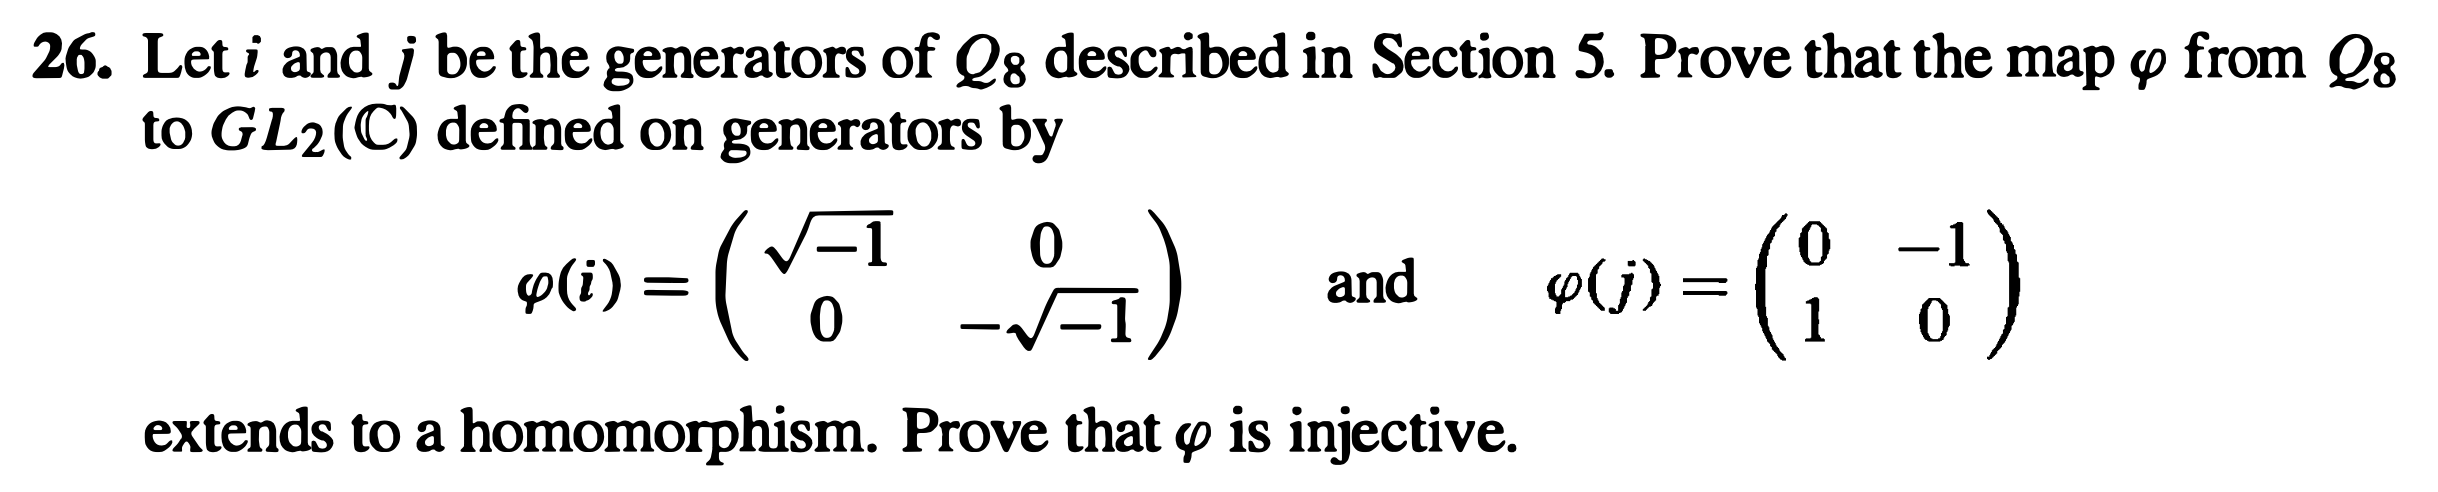
\includegraphics[width=400pt]{img/abstract-algebra--nf--3-1a71.png}
\end{mdframed}

\begin{proof}
  A presentation for $Q_8$ is
  \begin{align*}
    Q_8 = \big\langle i, j ~\big|~ i^2 = -1, ~ i^3 = -i, ~ i^2j = -j, ~ ij = k, ~ i^3j = -k \big\rangle.
  \end{align*}
  Let $\alpha = \sqrt{-1} \in \C$, and let $I \in GL_2(\C)$ be the identity matrix, and extend
  $\varphi$ to $k$ by
  \begin{align*}
    \varphi(k) &= \varphi(i)\varphi(j) = \matMMxNN{\alpha}{0}
                                 {0}{-\alpha} \matMMxNN{0}{-1}
                                                  {1}{0} = \matMMxNN{0}{-\alpha}
                                                                    {-\alpha}{0} \\
  \end{align*}

 We see that
  \begin{align*}
    \varphi(i)^2 &= -I \\
~\\
    \varphi(i)^3 &= -iI \\
~\\
    \varphi(i)^2\varphi(j) &= -I \matMMxNN{0}{-1}
                             {1}{0} = \matMMxNN{0}{1}
                                               {-1}{0} = -\varphi(j) \\
~\\
    \varphi(i)\varphi(j) &= \varphi(k) \\
~\\
    \varphi(j^2) &= \matMMxNN{0}{-1}
                      {1}{0}^2 = \matMMxNN{-1}{0}
                                          {0}{-1} = -I \\
  \end{align*}


  Note that we can write an arbitrary element $x \in Q_8$ as $x = i^aj^b$ for
  some $a, b \in \{0, 1, 3\}$:
  \begin{align*}
    1,~ -1 = i^2,~ i,~ -i = i^3,~ j,~ -j = i^2j,~ k = ij,~ -k = i^3j.
  \end{align*}



  We must show that $\varphi$ defined as above on $i$ and $j$ can be extended such
  that $\varphi(xy) = \varphi(x)\varphi(y)$ for all $x, y \in Q_8$.

  Let $\alpha = \sqrt{-1} \in \C$, and let $I \in GL_2(\C)$ be the identity matrix, and define $\varphi$ by

  \begin{align*}
    1 &\mapsto I \\
    ~\\
    -1 &\mapsto -I\\
    ~\\
    i &\mapsto \matMMxNN{\alpha}{0}
                  {0}{-\alpha} \\
    ~\\
    -i &\mapsto \matMMxNN{-\alpha}{0}
                   {0}{\alpha} \\
    ~\\
    j &\mapsto \matMMxNN{0}{-1}
                  {1}{0} \\
    ~\\
    -j &\mapsto \matMMxNN{0}{1}
                   {-1}{0} \\
    ~\\
    k &\mapsto \matMMxNN{0}{-\alpha}
                   {-\alpha}{0} \\
    ~\\
    -k &\mapsto \matMMxNN{0}{\alpha}
                   {\alpha}{0}
  \end{align*}

  We see that
  \begin{align*}
    \varphi(i)^2 = \varphi(j)^2 = -I
    \varphi(i)^2 &= \matMMxNN{\alpha}{0}
                      {0}{-\alpha}^2 = \matMMxNN{-1}{0}
                                           {0}{-1} = -I \\
    \varphi(j^2) &= \matMMxNN{0}{-1}
                      {1}{0}^2 = \matMMxNN{-1}{0}
                                          {0}{-1} = -I \\
  \end{align*}



  Thus $\varphi(xy) = \varphi(i^aj^bi^cj^d)$ for some $a, b, c, d \in \{0, 1, 3\}$.




\end{proof}
